\documentclass[a4paper,10pt]{scrreprt}
\usepackage[utf8]{inputenc}
\usepackage[T1]{fontenc}
\usepackage[french]{babel}
\usepackage{csquotes}
\usepackage{graphicx}
\usepackage[margin=1.2in]{geometry}

\usepackage{xcolor}
\usepackage{titlesec}
\usepackage{lmodern}% just for the example
\usepackage{lipsum}% just for the example

\colorlet{ctcolorchapterline}{black}
\colorlet{ctcolorchapternum}{black}

\newcommand\mychapformat[1]{%
  \parbox[b]{\dimexpr\textwidth-3em\relax}{\raggedright#1}}
\titleformat{\chapter}[display]%
  {\usekomafont{chapter}\sectfont}%
  {\vspace{-8em}\raggedleft{%
    {\color{ctcolorchapterline}%
        \rule[-5pt]{2pt}{5cm}}\quad%
    {\color{ctcolorchapternum}
        \fontsize{60}{60}\selectfont\thechapter}%
    }%
  }%
  {-2.1em}%
  {\mychapformat}%
  [\phantomsection]


\usepackage[backend=biber]{biblatex}
\bibliography{bibfile}

\usepackage[hidelinks]{hyperref}

\usepackage{siunitx}
\usepackage{bm}
\usepackage{amsmath}

\title{PAM Synthèse hybride d'instruments à cordes}
\author{Théis Bazin, Louis Moreau-Gaudry, Victor Rosi \\ Hugo Caracalla et Maxime Dickerson}

\begin{document}
\maketitle

\Introductionbegin{frame}{Introduction}
  
\beamerdefaultoverlayspecification{} % Regardez pas ça, c'est juste pour
% temporairement pas faire le dévoilement pas-à-pas.

	\begin{itemize}
	  \item Synthèse hybride: inclusion de mesure dans la synthèse sonore
	  \item Interets: 
	  \begin{itemize}
	     \item temps de calcul (vs Méthodes Numériques)
	     \item aide à la facture
	  \end{itemize}
	\end{itemize}

\end{frame}


\chapter{Mesures d'admittances sur instruments à cordes pincées}
Dans cette partie nous procédons à la mesure d'admittance (accélération sur force) d'une guitare et d'un Ukulélé au niveau du point de couplage entre la corde et le corps.
\section{Nomenclature des grandeurs physiques :} 
\begin{itemize}
\item $Y_{body,indices}$ : Admittance du corps. l'indice $1$ indique l'axe vertical et l'indice $2$ l'axe horizontal.
\item $Y_{string,indices}$ : Admittance de la corde.
\item $Y_{total,string,indices}$ : Admittance de l'ensemble corde+corps.
\item $y_{string,wire}$ : signal temporel de la corde excitée au fil.
\item $F$ : Force appliquée par le marteau 
\item $\alpha$ : Accélération délivrée par le capteur 
\end{itemize}

\section{Dispositif de mesure employé}
Pour nos mesures, nous disposons de : un capteur tri-axes,
un marteau d'impulsion, une carte d'acquisition NI, un amplificateur,
un système d'acquisition sur Matlab, un microphone, une guitare.
En amont de nos mesures, nous renseignons la fréquence d'échantillonnage et la sensibilité du capteur dans le code d'acquisition. Le marteau d'impulsion fourni la force d'impacte $F$ sur la guitare. 

Lors de l'acquisition de nos résultats, le signal d'impulsion du marteau est fenétré dans le temps autour de son attaque dans le but d'eliminer le bruit électronique, dont on veut ignorer l'influence. 

Au final nous récupérons, la réponse temporelle de l'accélération en 2D et de la force. On obtient également leur réponse fréquentielle, c'est le rapport des deux, qui donne l'admittance du système.

L'installation du banc de mesure est présenté en Annexe. %dans la Figure \ref{fig:gull}.

%\begin{figure}[h]
%centering
%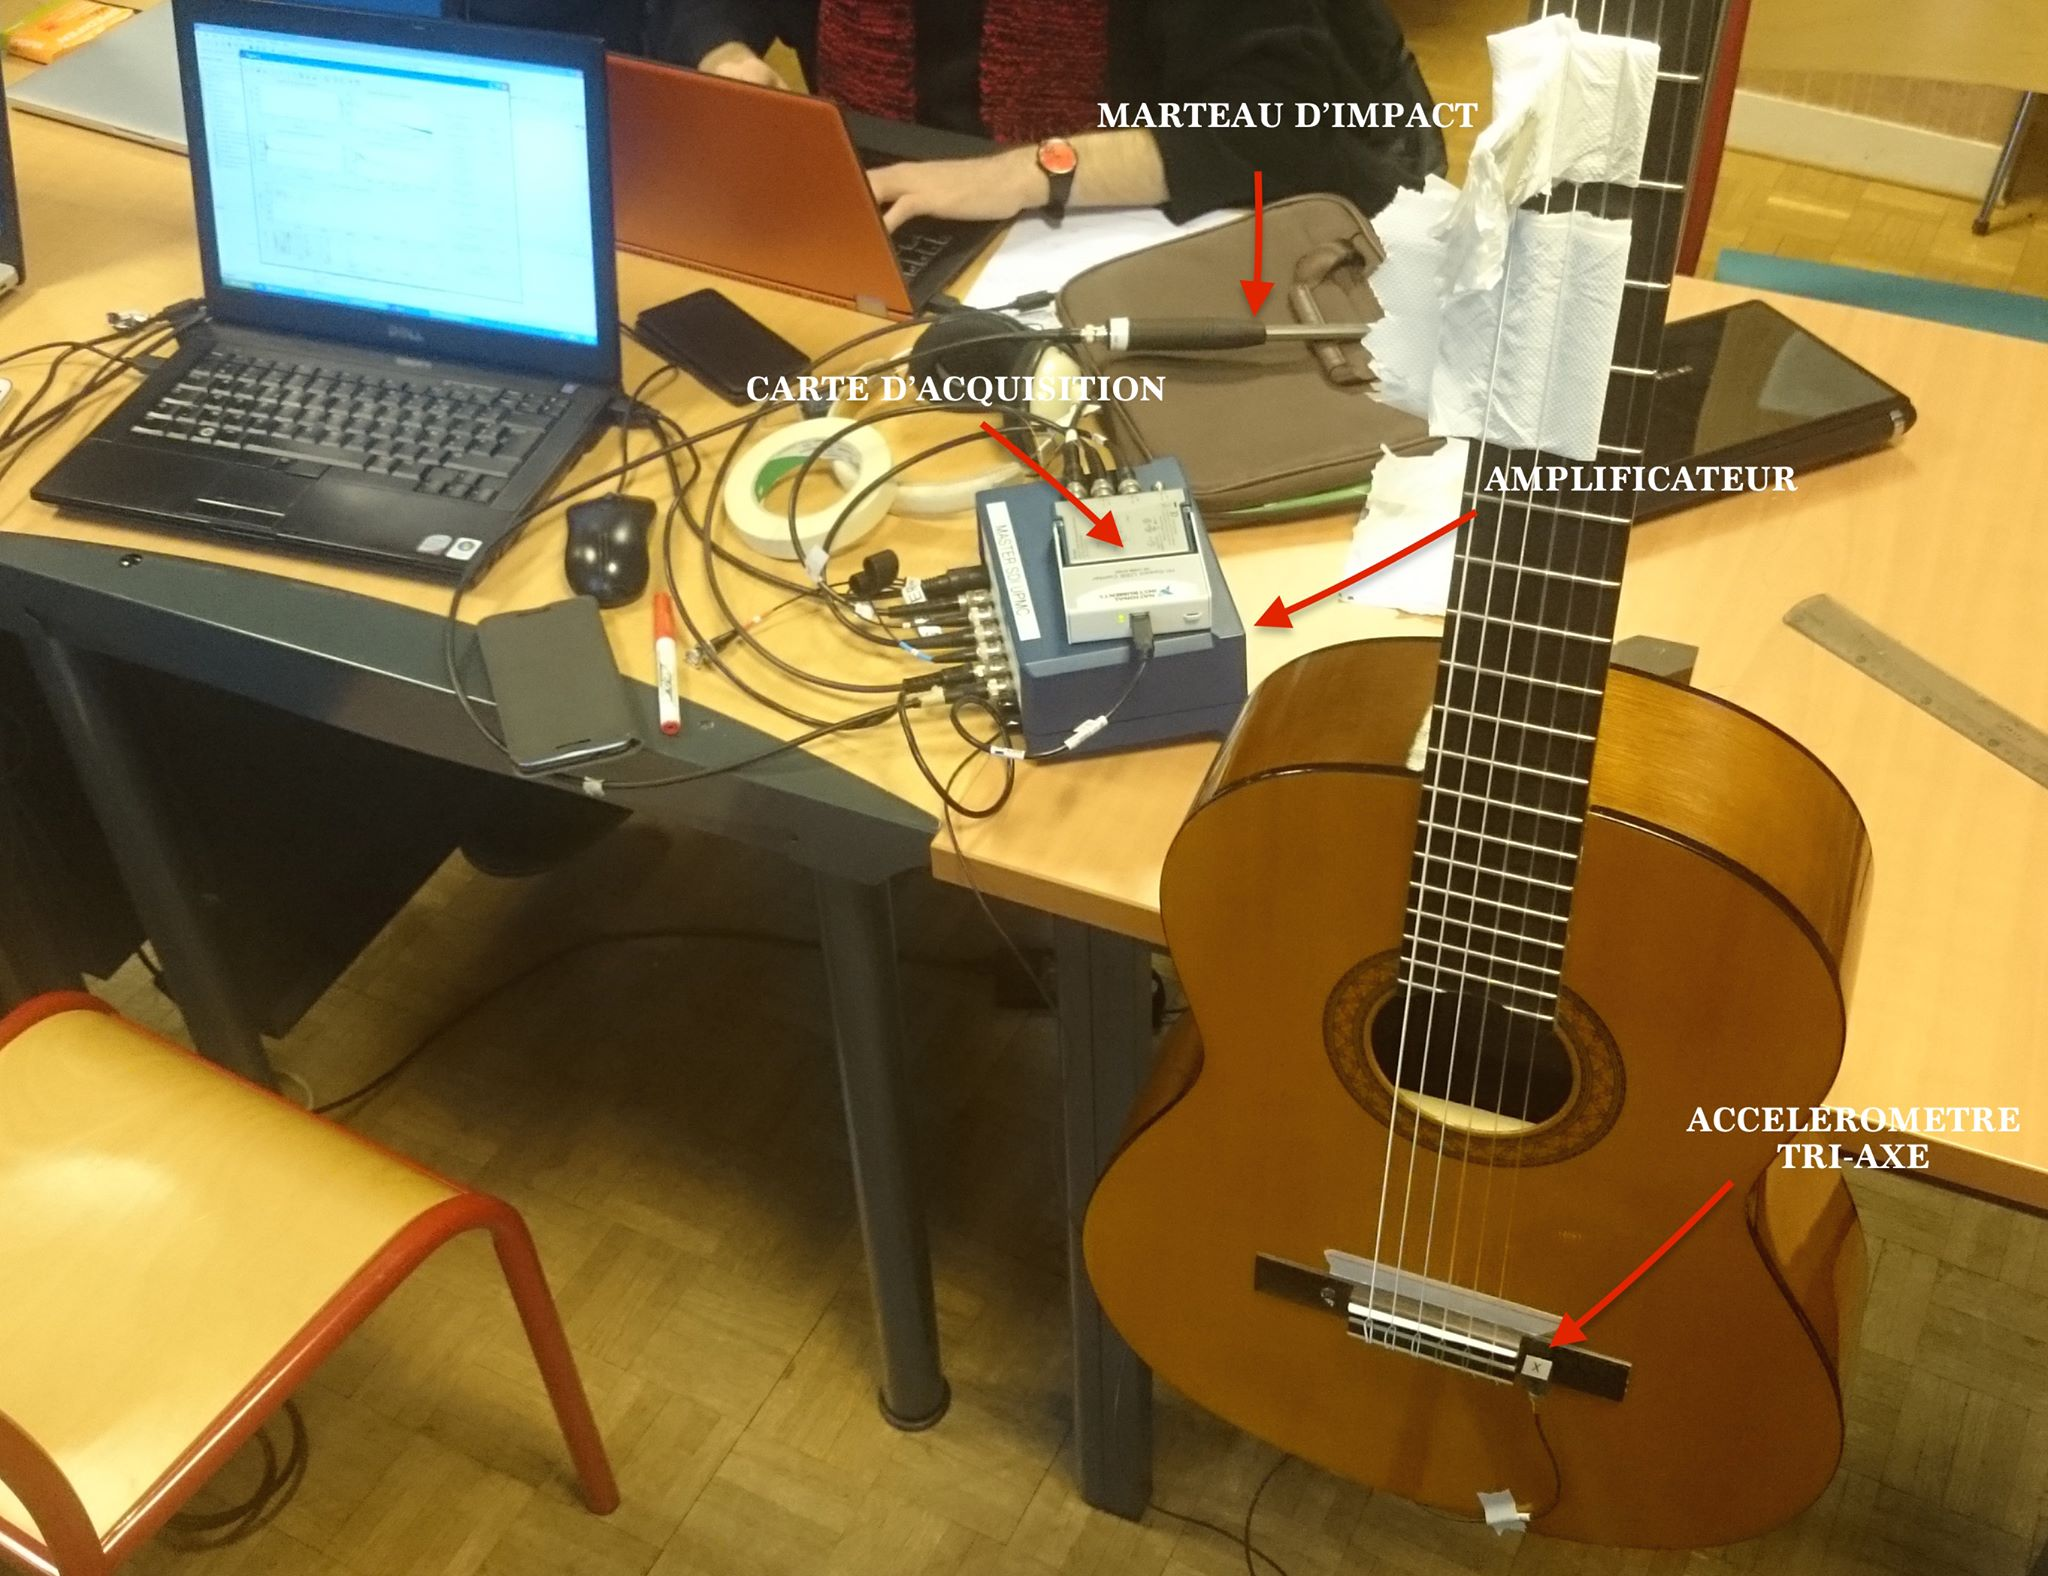
\includegraphics[width = 7cm]{dispo.JPG}
%\caption{Dispositif de mesure}
%\label{fig:gull}
%\end{figure}

\section{Protocole de mesures}
Voici l'ensemble des mesures effectuées. Pour assurer une répétablité de la mesure, elles seront faites 5 fois chacune dans le même temps. Nous choisissons une valeur de fréquence d'echantillonnage pour l'accéléromètre de  $F_e = \si{25600\Hz}$.
\begin{itemize}
\item Le corps seul, axe vertical(les cordes sont étouffées).
\item Le corps et la corde de \( E2 \), axe vertical et horizontal.
\item Le corps et la corde de \( E4 \), axe vertical et horizontal.
\item La corde \( E4 \) excitée au fil perpendiculairement à la table.
\item La corde \( E4 \) excitée au fil à \( \si{45 \degree} \) de la table.
\item Mesure du rayonnement de la table seule.
\end{itemize}
Les deux dernières mesures consistent en l'excitation de la corde avec un fil de cuivre à une distance b = 17 mm du chevalet. 

\section{Commentaire et exploitation des résultats}
\subsection{Visualisation des résultats}
La Figure \ref{fig:goll} montre l'ensemble de nos résultats d'admittance pour le corps seul, mesuré au niveau de la corde de \( E4 \).

\begin{figure}[hpbt]
\centering
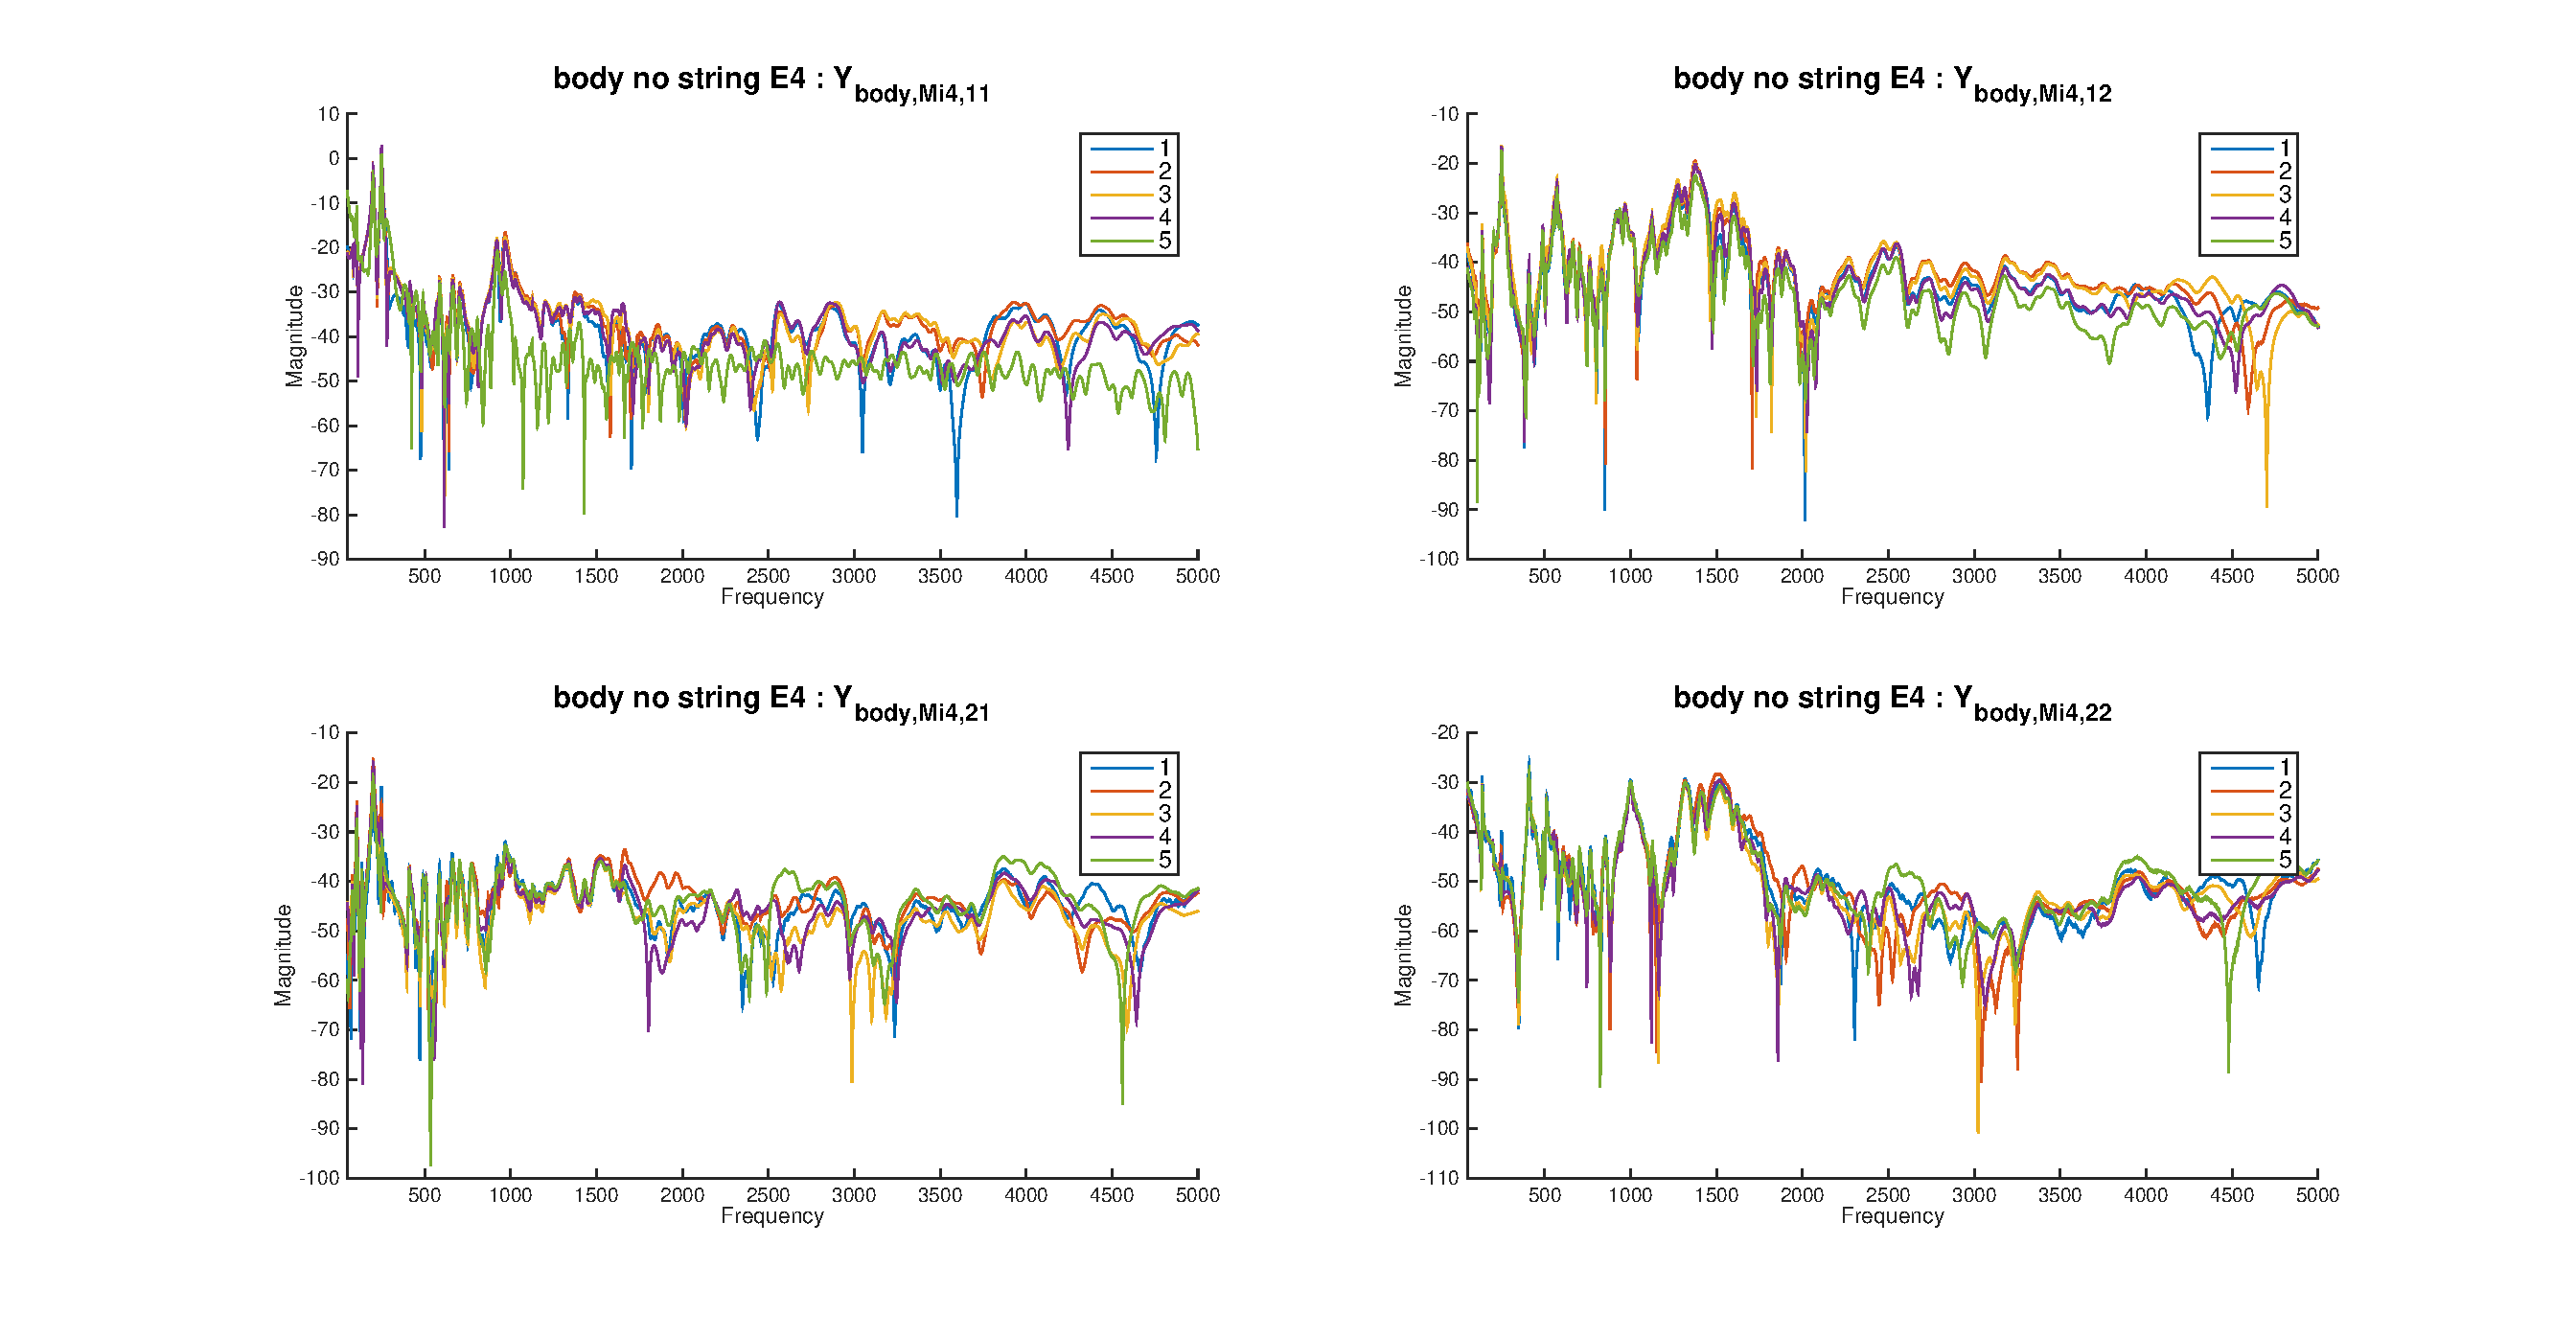
\includegraphics[width = \linewidth]{figures/Y_body_E4.eps}
\caption{Mesures pour le corps au niveau du chevalet et de la corde de \( E4 \)}
\label{fig:goll}
\end{figure}

La première ligne correspond à la mesure avec impulsion normale à la table, la seconde ligne, à une impulsion parallèle. On obtient deux dimensions de l'admittance pour ces mesures, effectuées 5 fois chacune. Pour nos synthèses, nous ne nous servirons que de l'admittance correspondant au déplacement transversal de la table ($Y_{body,11}$, $Y_{body,12}$ et $Y_{body,21}$) doivent être semblable.

\subsection{Calcul de la cohérence}
Dans le but de juger de la viabilité de nos mesures, nous calculons la cohérence des 5 mesures de $Y_{body,11}$ au niveau de la corde de \( E2 \) et de la corde de \( E4 \). La Figure \ref{fig:goll},  montre dans le graphe de $Y_{body,11}$ une mesure (la 5ème) que nous pourrons ignorer dans ce calcul. Les chutes locales de cohérence observées avant \( \si{2000\Hz} \) sont généralement dues à des anti-résonances autour desquelles les valeurs très faibles mesurées peuvent être assimilées à un bruit statistique.


\begin{figure}[hpbt]
\centering
\begin{tabular}{cc}
   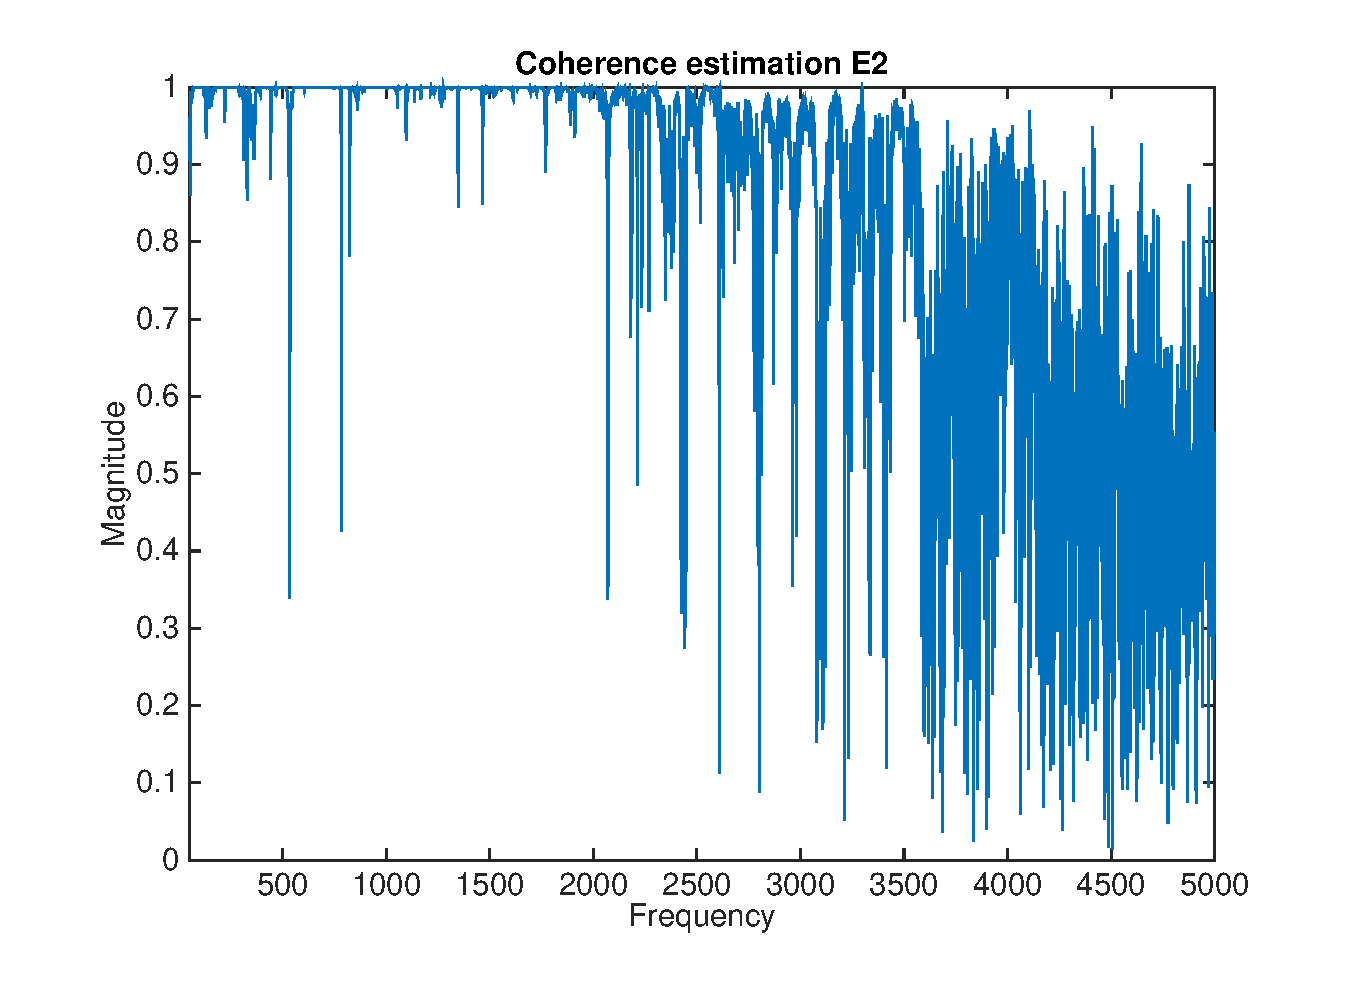
\includegraphics[width = 5cm]{figures/coherence_Z_1_E2.eps} &
   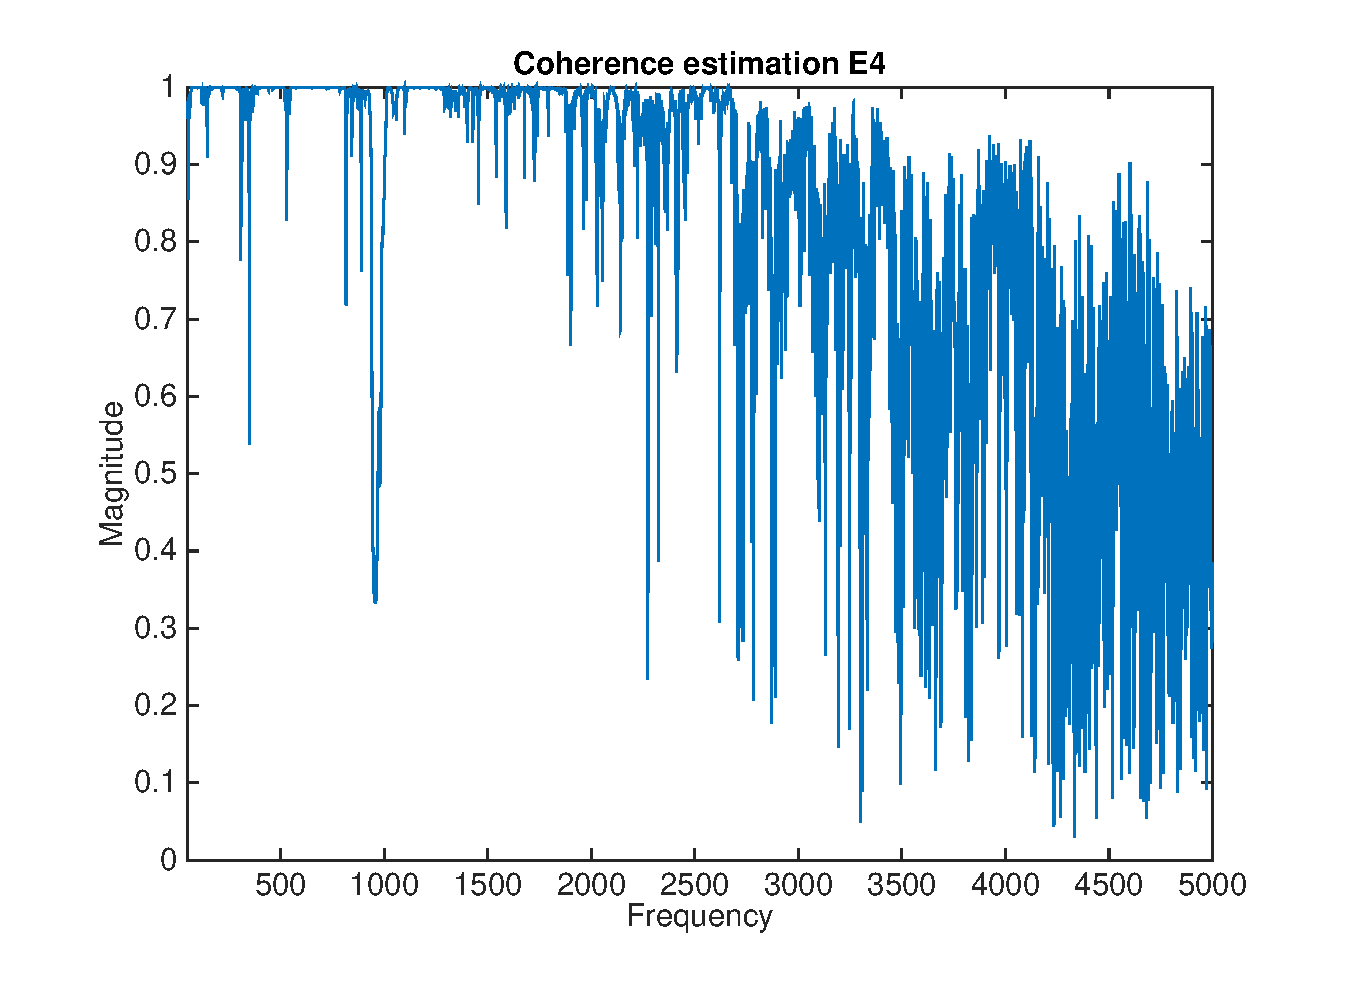
\includegraphics[width = 5cm]{figures/coherence_Z_1_E4.eps} \\
\end{tabular}
\caption{Cohérence des mesures Ybody1 au niveau de la corde de \( E2 \) et de celle de \( E4 \)}
\label{fig:gall}
\end{figure}
Nous observons sur la Figure \ref{fig:gall} une baisse importante de la cohérence autour de la fréquence de \( \si{2000\Hz} \). Cela est dû à un filtrage passe-bas du marteau qui ne produit pas une impulsion parfaitement ponctuelle lors de l'excitation. Nous pourrons donc dans nos synthèse, limiter notre recherche des modes de corps à la région fréquentielle entre \( \si{0} \) et \( \si{2000\Hz} \).

\section{Extraction des paramètres}

Une fois la qualité des mesures évaluée, il s'agit maintenant d'en extraire les paramètres nécessaires à la fois à la synthèse par FRF et à la synthèse modale.

\subsection{Paramètres de synthèse FRF}

Dans le cadre de la première, l'admittance $Y_{body}$ du corps sans corde de l'instrument est obtenue de façon directe au travers des mesures de la partie précédente : ne restent à être extraites uniquement les valeurs des fréquences de résonance de la corde et celles de leurs amortissements.\\

Pour ce faire, et en se basant sur la relation [REF NEEDED], il est en théorie possible de commencer par extraire $Y_{string}$ des valeurs mesurées de $Y_{body}$ et $Y_{total}$ puis d'analyser $Y_{string}$ et d'identifier au moyen de la relation [REF NEEDED] les fréquences et amortissements. Malheureusement il existe entre l'admittance de corde et les deux autres une différence d'ordre de grandeur telle que les simple bruit de mesure de ces dernières noie le signal qui aurait du être $Y_{string}$ : cela nous pousse donc à la mesurer directement sur banc de corde, ce qui par manque de temps ne sera pas fait au cours de ce projet. La suite de cette partie s'attache cependant à mettre en place un protocole d'extraction des fréquences et amortissement en supposant la connaissance de $Y_{string}$.\\

\subsubsection{Analyse ESPRIT par bandes}
\label{esprit}

Supposons donc que nous disposions d'une admittance $Y$, issue d'une mesure sur corde : il est donc à priori possible, en extrayant sa fréquence fondamentale via produit spectral, puis en recherchant chaque harmonique sur une plage de fréquence dictée par les valeurs des harmoniques précédents, d'obtenir une première série de valeurs de fréquences de modes. Cette méthode n'a cependant pas le mérite d'être très précise, et ne renvoie pas non plus de valeurs d'amortissement : elle peut cependant servir de base à une analyse par méthode à haute-résolution (dans le cas présent, la méthode ESPRIT [REF NEEDED]) centrée autour de ces premières approximations de fréquences.\\
Le signal est dans un premier temps filtré autour de chacun de ces harmoniques par filtre passe-bande à réponse finie et phase linéaire, ceci afin de garantir des signaux filtrés présentant les mêmes pôles que le signal d'origine (le résultat est visible en [REF NEEDED]). Afin d'accélérer l'analyse par méthode ESPRIT, il est ensuite modulé par la fréquences de l'harmonique approximatif afin de la recentrer autour de $0 Hz$ (voir [REF NEEDED]) et de permettre une décimation (voir [REF NEEDED]). S'ensuit alors une analyse par ESPRIT, qui donne directement accès aux valeurs exactes de fréquences propres et amortissement de $Y$.

\begin{figure}[h]
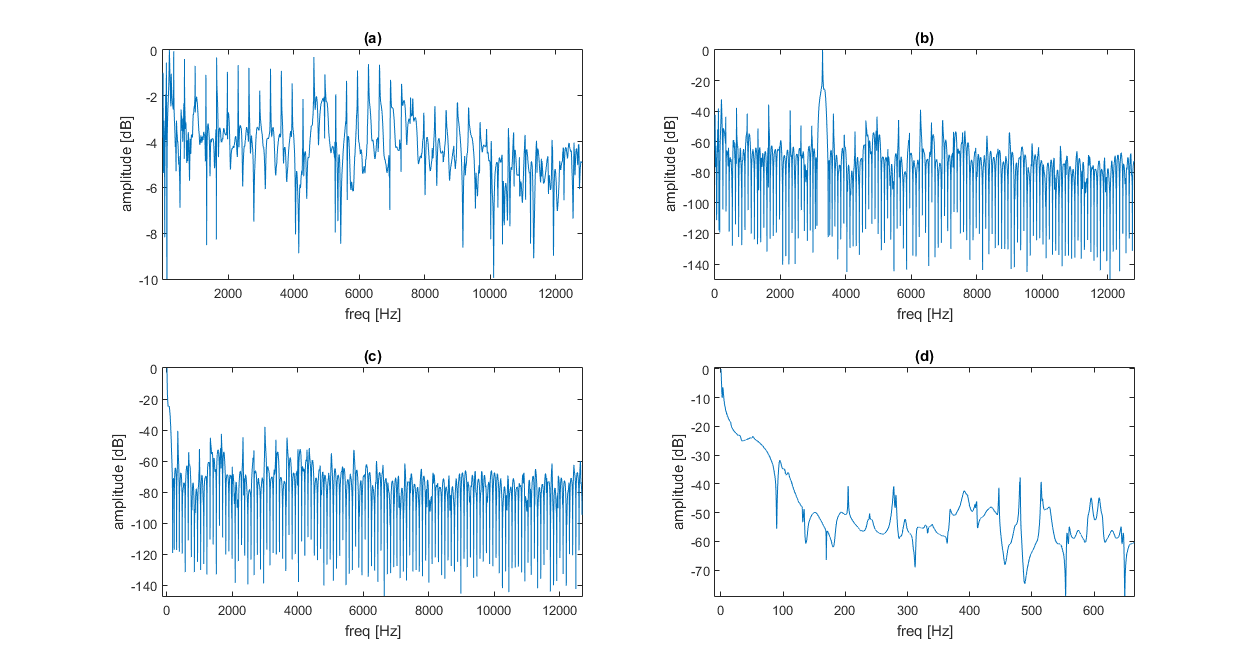
\includegraphics[scale=0.5]{figures/pre_proc.png}
\caption{\textit{(a) spectre du signal d'entrée - (b) spectre du signal filtré sur un harmonique - (c) spectre du signal modulé par la fréquence de l'harmonique - (d)spectre du signal décimé.}}
\label{pre_proc}
\end{figure}

\subsubsection{Valeurs utilisées}

A défaut d'utiliser ce protocole pour extraire les paramètres de la synthèse par FRF, les valeurs fournies par Woodhouse [REF NEEDED] seront utilisées.

\subsection{Paramètres de synthèse modale}

Les paramètres utilisés en entré de la synthèse modale sont des paramètres physiques, notamment :
\begin{itemize}
 \item Tension \( T \), raideur de flexion \( B \), longueur \( L \) et
  masse linéique \( \rho \) pour la corde,
 \item Facteurs de qualité pour les modes de corde et de corps en isolation,
 \item Admittance de corps pour calculer les masses effectives,
 \item Fréquences propres et amortissements pour les modes de corps.
\end{itemize}
N'ayant pu les mesurer pour la plupart, nous utiliserons des valeurs pour
partie fournies par Woodhouse dans son article de mesures,
% (\( T, B, L, \rho \)),
% pour partie calculées par des modèles théoriques
% proposés par Woodhouse (facteurs de qualité de la corde)
ou des valeurs mesurées.
\\\\

Les paramètres ayant été rassemblés, il est maintenant possible de produire par chacune des méthodes de synthèses un son dont les conditions initiales sont contrôlées.

\section{Analyse des résultats}
Afin de pouvoir comparer les résultats de synthèse à un signal réel obtenu par mesure, nous utilisons $y_{string,wire}$ comme référant et implémentons ses conditions initiales (à savoir une impulsion de force à une distance donnée du chevalet) dans nos deux algorithme de synthèse.\\
Afin de comparer les signaux de synthèse au signal mesuré, il est entièrement possible d'utiliser le protocole développé en partie \ref{esprit} afin d'extraire les paramètres de de signaux de corde et qui renvoyait les valeurs des fréquences de résonances et leurs atténuation.\\

\begin{figure}[h]
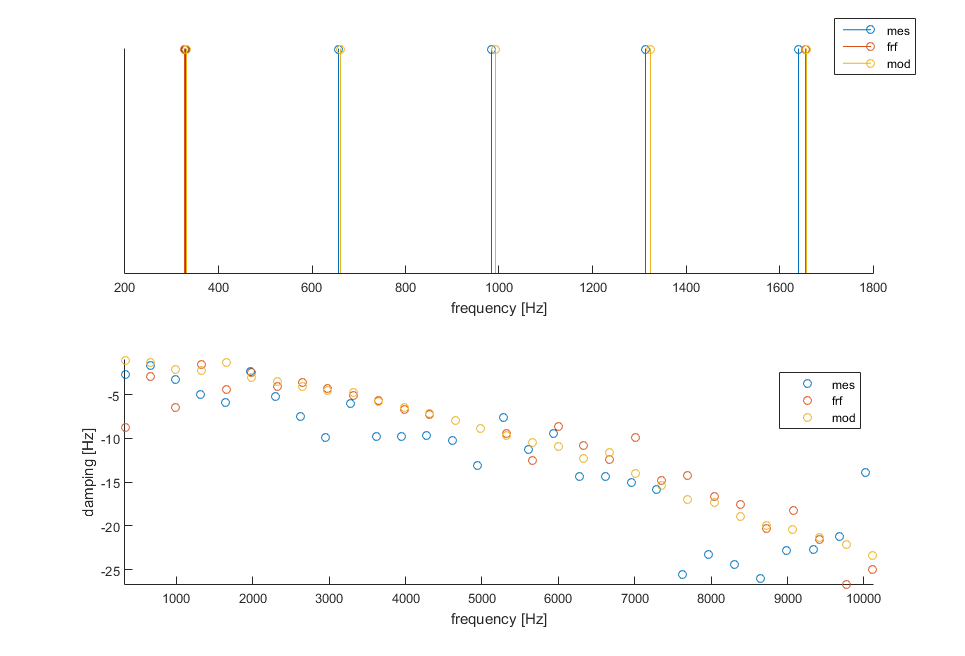
\includegraphics[scale=0.65]{figures/apotheose.png}
\caption{\textit{haut-dessus : tracé des fréquences de résonances des différents signaux (synthèses et réel); en-bas : tracé des atténuations en fonction des fréquences de résonance.}}
\label{apo}
\end{figure}

Les résultats de ces extractions de paramètres sont visibles en figure \label{apo}. Les fréquences des deux méthodes de synthèses restent identiques, même en haute-fréquences, mais différent peu à peu de la fréquence du signal réel : cela peut être compris comme étant due à l'inharmonicité intrinsèque de la corde réelle qui, au contraire de celle issue du couplage avec le corps, n'est pas prise en compte par nos modèles de corde. Les atténuations sont satisfaisantes, puisqu'elles décrivent la même allure décroissante que celle du signal réel.


\chapter{Syntèse}
\section{Synthèse FRF}

\subsection{Principe}
% méthode hybride ici. mélange mesures et théorie
\paragraph*{} 

Le principe de la synthèse dans le domaine fréquentiel est relativement simple.
Il s'agit de calculer ou de mesurer des fonctions de transfert
(\textit{Frequency Response Function}) nous permettant de relier une force
appliquée au point d'excitation de la corde à un déplacement au niveau du
chevalet, de la table d'harmonie de la guitare, ou d'un autre instrument comme le ukulélé. On parle de méthode hybride puisqu'elle conjugue modèles théoriques et mesures sur instruments. Le premier élément nécessaire est l'admittance au chevalet, qui peut s'exprimer grâce à l'admittance des cordes et celle du corps au niveau du chevalet (par corps, il faut comprendre la table d'harmonie et la caisse de la guitare), par l'équation \ref{eq:eq_frf_1}.\\

Cette admittance totale au niveau du chevalet nous fournit la vitesse de
celui-ci en fonction d'une force qui y serait appliquée. \\

Le second élément nécessaire est la fonction de transfert $H$ reliant un
déplacement de la corde à un déplacement au niveau du chevalet. En multipliant cette fonction avec $Y_{total}$, on obtient la FRF fournissant le déplacement $\delta_{excitation}$ en fonction de la force $F_{chevalet}$. Le système étant supposé linéaire, le principe de réciprocité de Betty s'applique et cette fonction de transfert fournit aussi le déplacement $\delta_{chevalet}$ en fonction de la force $F_{excitation}$ (équation \ref{eq:eq_frf_2}).


\subsection{Mise en place}
% implémentation
% H, Z, Ytotal
\subsubsection{Formulations théoriques}
L'article de Woodhouse à notre disposition nous permet d'écrire l'impédance
de la corde au chevalet $Z_{corde}$, ainsi que la fonction de transfert
unitaire $H$ à partir de la connaissance des caractéristiques de la corde :
masse linéique, tension, coefficients d'amortissement, raideur de flexion (équations \ref{eq:eq_frf_4} et \ref{eq:eq_frf_5}). Ces fonctions de transfert sont dépendantes de l'écriture des modes de corde et le modèle de leur amortissement choisi par Woodhouse est présenté à l'équation \ref{eq:eq_frf_4}.

\subsubsection{Mesures sur la guitare}
Les mesures sur les instruments fournissent une estimation de $Y_{corps}$ et de $Y_{total}$. \\

La première approche est d'utiliser uniquement $Y_{total}$ mesurée en
excitant au marteau d'impact un point proche du chevalet et en mesurant son accélération selon l'axe normal et l'axe transverse par rapport à la table
d'harmonie. La corde que l'on souhait synthétiser est libre de vibrer
alors que les autres sont étouffées. En réalité, nous mesurons l'inertance,
ce qui doit ajouter une seconde intégration à l'équation \ref{eq:eq_frf_2}.\\

La seconde approche est de n'utiliser que la mesure de $Y_{corps}$ .
L'admittance de la corde $Y_{corde}$ au chevalet utilise les formulations théoriques de l'article (équation \ref{eq:eq_frf_4}) pour obtenir $Y_{total}$. \\

\subsubsection{Implémentation}
Les FRF issues des mesures temporelles sont calculées avec un très grand nombre de points pour que le signal final dure plusieurs secondes. L'obtention du son est en effet réalisée par FFT inverse, ce qui nous impose d'écrire la symétrie hermitienne pour notre fonction de transfert pour assurer que le signal synthétisé est bien réel.

L'intégration de l'équation \ref{eq:eq_frf_2} fournit des valeurs en basses fréquences divergentes en zéro. Pour compenser cela nous intégrons dans le domaine fréquentiel en imposant des valeurs très faibles de la FRF en-dessous de 50 Hz (notre note la plus basse était un Mi grave de 83 Hz).

Enfin, nous convoluons ce signal avec une ou plusieurs impulsions consécutives pour adoucir le son par un filtrage passe-bas et modéliser une force qui dure dans le temps.

\subsection{Résultats}
%

Utiliser $Y_{total}$ mesuré ne fournit pas de résultats convaincants. Les sons synthétisés ne correspondent pas à ceux d'une guitare. Woodhouse suggère en effet d'effectuer la séparation de cette grandeur, ce que nous avons choisi de faire exclusivement.\\

Toutes les cordes à vide de la guitare sont synthétisées, avec comme excitation une force ponctuelle et une force qui dure dans le temps, ceci pour chaque mesure d'amittance à notre disposition. La partie théorique de cette synthèse utilise 40 modes de cordes, et les sons obtenus durent 11 secondes. On reconnait clairement un son de guitare à l'écoute. Voici une des fonctions de transfert obtenues de notre système :

\begin{figure}[h]
\centering
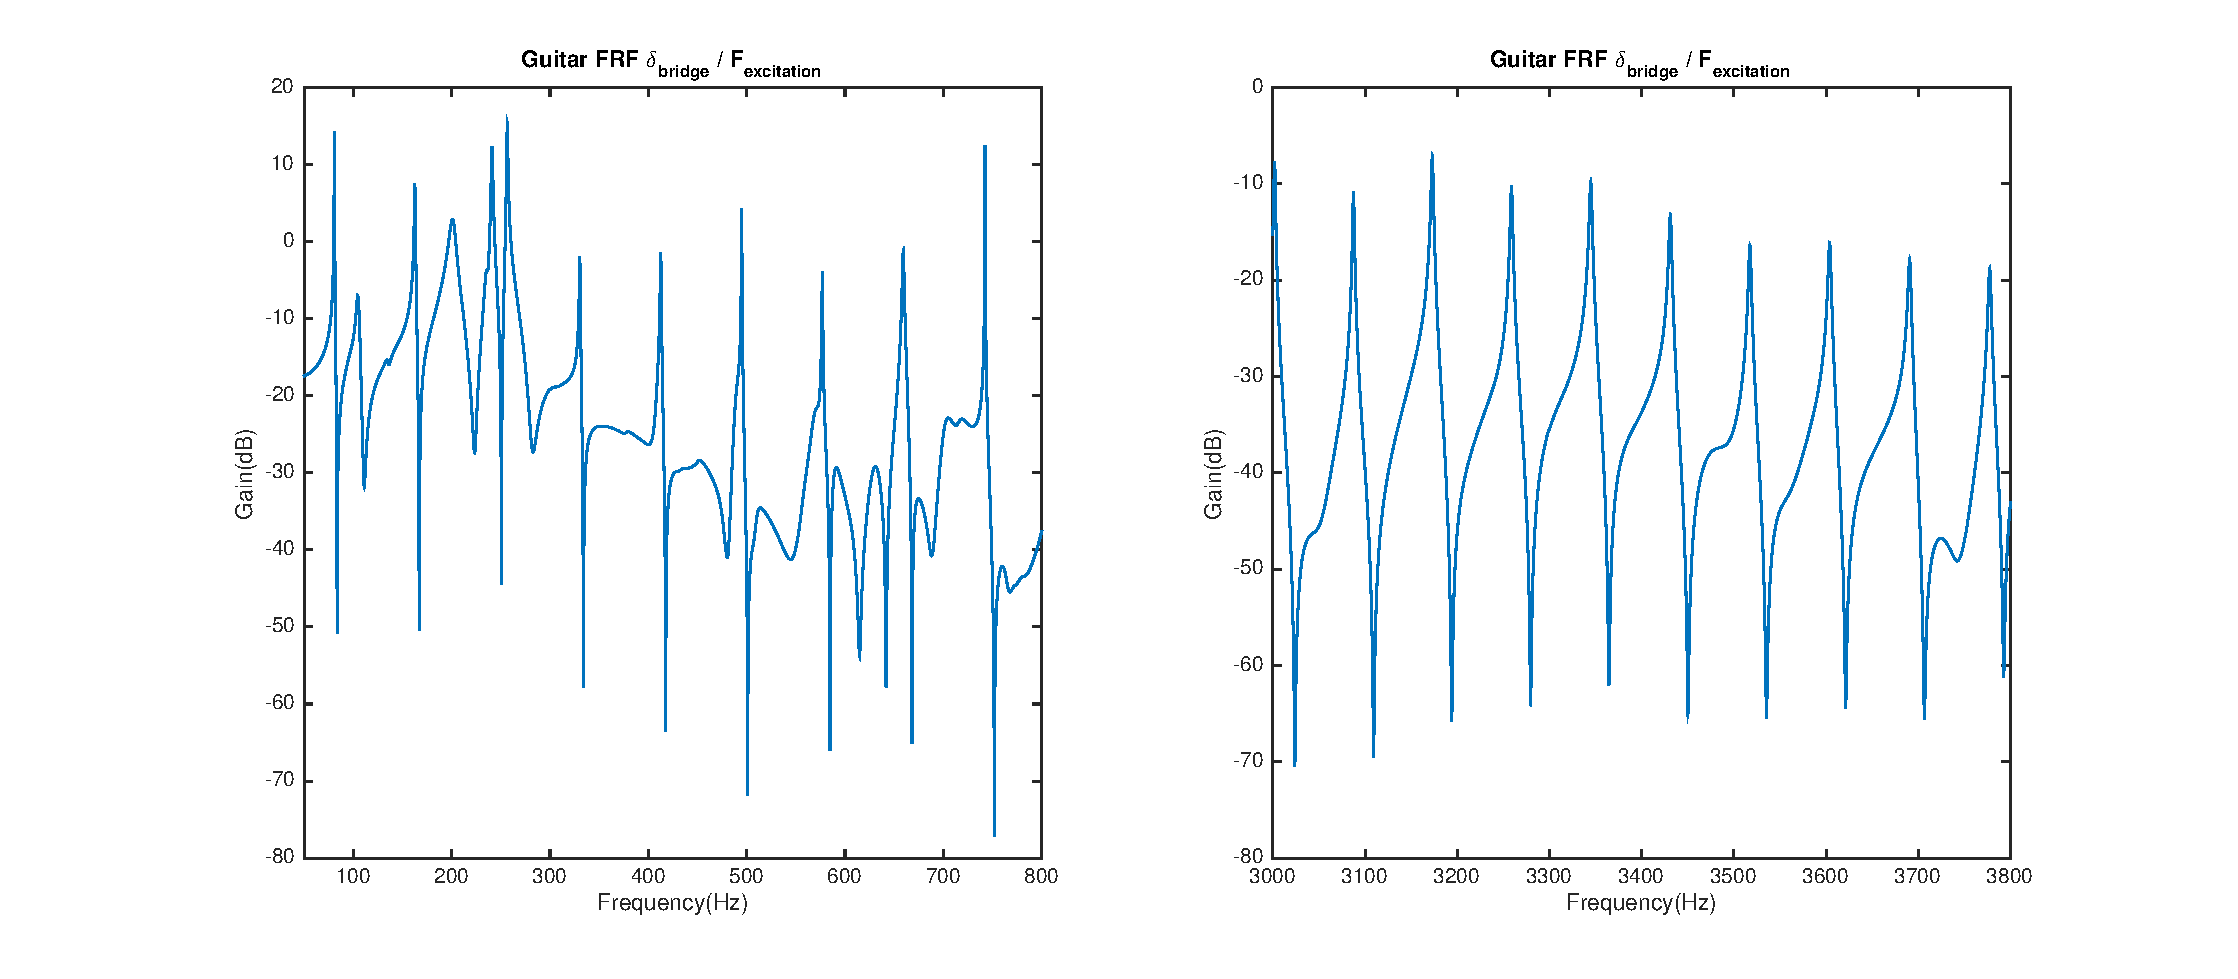
\includegraphics[width=\linewidth]{../figures/FRF_E2.eps}
\caption{Admittance de la synthèse hybride}
\label{fig:frf_fig_1}
\end{figure}


Plusieurs précisions ont du être apportés pour améliorer l'algorithme et le
son. En effet, ce système comporte plusieurs limitations : l'admittance
$Y_{corps}$ est affectée par la présence de cordes même atténuées. Cet effet est difficilement écarté puisqu'ôter les cordes de l'instrument modifie la masse au niveau du chevalet. Aussi, nous n'avons pas mesuré les caractéristiques des cordes de la guitare à notre disposition mais nous sommes basés sur des valeurs fournies par Woodhouse, qui peuvent ne pas correspondre à notre instrument.\\


%
%
% $c$ pour chevalet, $e$ pour excitation.
% $$\frac{1}{Y_{tot}} = \frac{1}{Y_{corps}} + \frac{1}{Y_{corde}}$$
%$$F_c \times Y_{tot} = v_c$$
%$$v_c \times \tilde{H} = v_e$$
%$$\frac{v_e}{j\omega} = \delta_e$$
%par théorème de réciprocité de Betty : 
%$$\frac{\delta_c}{F_e} = \frac{\delta_e}{F_c} = \frac{Y_{tot}\tilde{H}}{j\omega}$$
%
%


\section{Synthèse modale}

\paragraph{}
  On présente dans cette partie le processus d'analyse/synthèse modale hybride
appliqué dans le cadre du projet. Ce processus est basé sur les principes
suivants : les paramètres physiques découplés de corde et de guitare sont
posés, pour la corde via un modèle théorique, pour le corps en appliquant
\textsc{esprit} sur les mesures d'admittance effectuées et en remontant aux
paramètres physiques du système.
  Ensuite, le système d'équations différentielles à \( N \) modes du système
couplé est posé et on résout ce système pour en extraire les déformées modales
et les fréquences propres du système couplé. Enfin, en posant fixant des
conditions initiales, on peut resynthétiser le son de la corde couplée au
chevalet.

\subsection{Paramètres physiques}

\paragraph{}
Par souci de concision, on ne présente pas dans ce rapport le détail des
matrices développées dans l'article de Woodhouse, mais seulement la façon dont
les paramètres physiques pertinents sont extraits ou fixés.

\subsubsection{Corde}
  \paragraph{}
  La corde suit un modèle théorique basé sur sa longueur \( L \), sa tension
\( T \), sa raideur de torsion \( B \) et sa masse linéique \( \rho{} \).
  On choisit ensuite le nombre de modes de corde désiré.
  Pour une corde de Mi grave (\( E2 \)), dont la fréquence fondamentale est
de \( \si{82.4 \hertz}\), le \( 39 \)ème harmonique aura une fréquence (modulo 
inharmonicité) proche de \( \si{3214\hertz} \), c'est la valeur maximale que
l'on fixe.

  Concernant les conditions aux limites, la corde est supposée fixe-fixe
en isolation et le couplage est ensuite réalisé au niveau du chevalet à l'aide
d'un mode de contrainte rigide qui permet d'inclure les vibrations du corps.

\subsubsection{Corps}

  \paragraph{}
  Les paramètres physiques du corps sont extraits par analyse modale via ESPRIT.
Dans l'état actuel, nous ne suivons pas complètement le processus proposé par
Woodhouse, qui ne fait de l'analyse modale que jusqu'à \( \si{1500\hertz} \)
puis, dans la partie haute-fréquences, pose un modèle de répartition modale
statistique.
Notre version souffre d'un overfitting dans les basses-fréquences, on se limite
donc à un nombre restreint de modes de corps pour éviter cet overfitting.

  Une fois les fréquences propres et les amortissements du corps isolé
extraites, on en déduit les paramètres physiques du corps au niveau du
chevalet, modélisé comme un ensemble unidimensionnel de systèmes masse-ressorts
à \( N_b \) modes, d'admittance :
  \[ Y(\omega) = \sum_{k=1}^{N_b} \frac{j\omega{}}
    {m_k(\omega_k^2 + 2 j \omega{} \omega{}_k \xi{}_k - \omega{}^2)} \]
    
Pour ce faire, on définit pour chaque mode calculé une masse effective
\( m_k \) et une raideur effective \( s_k \) ainsi définies :

  Les masses modales sont obtenues par inversion locale autour de
\( \omega = \omega_k \) de l'expression de l'admittance~\cite{pate14:phd} et
valent \[ m_k = \frac{1}{2 |Y(\omega_k)| \omega{}_k \xi{}_k} \] une valeur plus
simple à calculer que celle proposée par Woodhouse -- son expression suppose de
connaître les déformées modales du corps.

  Les raideurs effectives en sont directement déduites et valent
\( s_k = m_k \omega{}_k^2 \), valeur qui permet d'assurer la vibration du système
à la pulsation \( \omega{}_k \).

\subsubsection{Couplage par équations différentielles matricielles}

  \paragraph{}
  L'étape suivante est la définition du système d'équations différentielles
cou\-plées. On se place dans la base des modes propres découplés de corde et de corps,
avec \( N_s \) modes de corde et \( N_b \) modes de corps. On a donc
pour vecteur de coordonnées le vecteur
  \( \bm{q}(t) = [a_1(t), a_2(t), \dots a_{N_s}(t),
    b_1(t), b_2(t), \dots, b_{N_b}(t)] \) de dimension
\( N = N_s + N_b \).
% , où les valeurs \( a_k(t) \) sont les amplitudes (variables
% dans le temps) des \( N_s \) modes de cordes modélisés et les \( b_k(t) \)
% celles des modes de corps retenus.

  L'équation différentielle matricielle du second ordre décrivant le système
couplé soumis à une excitation \( \bm{F} \) s'écrit alors
  \[ \label{eq:diff_second}
    M \ddot{\bm{q}} + C \dot{\bm{q}} + K \bm{q} = \bm{F} \]

  Les valeurs des matrices \( M \) et \( K \), respectivement de masse et de
raideur, sont obtenues dans l'article de Woodhouse par une analyse énergétique
du système et une inversion des résultats obtenus (une sorte de fitting
modal).

  L'amortissement est supposé (hypothèse simplificatrice choisie par Woodhouse)
visqueux (i.e. proportionnel pour chaque mode découplé à sa vitesse) et la
matrice d'amortissement \( C \) est donc diagonale dans la base des
modes découplés.

  Enfin, en supposant \( M \) inversible et en posant le vecteur
\( \bm{p} = \begin{pmatrix} \bm{q} \\ \bm{\dot{q}} \end{pmatrix} \) et la
matrice \( A = \begin{pmatrix} 0 & I \\ -M^{-1}K & -M^{-1}C \end{pmatrix} \)
(entachée d'erreur dans l'article de Woodhouse, ce qui a été la cause de pas
mal de tracas avant que nous ne nous en rendions compte\dots), on réécrit
\ref{eq:diff_second} comme une équation différentielle du premier ordre :
\[ \bm{\dot{p}} = A\bm{p} \]

\paragraph{}
  Les modes propres du système couplé alors obtenus en extrayant les valeurs
propres et une base de vecteurs propres de \( A \).

\section{Synthèse modale}

  La synthèse modale est effectuée selon des formules décrites
dans le livre de~\textcite{newland}, qui traduisent une sommation des modes
pondérée par les amplitudes issues des conditions initiales.

  La condition initiale choisie est actuellement un déplacement triangulaire
de la corde, avec prise en compte d'une largeur de doigt (d'un \( \si{\cm} \))
qui opère comme un filtre passe-bas.

\subsection{Statut de l'implémentation et observation de résultats}

Les valeurs requises ayant été obtenues comme décrit dans le chapitre suivant,
l'implémentation de la synthèse modale hybride est pleinement fonctionnelle
et efficace (moins de 10 secondes de calcul au total, calcul des paramètres
inclus, pour synthétiser 30 secondes de signal) et pourrait donc opérer en
temps réel.

Les résultats de la synthèse sont comparés avec les valeurs mesurées dans une
partie à venir.

On propose en Figure~\ref{fig:synth:modal_synth} la visualisation du résultat
de la synthèse du son de la corde \( E2 \) avec prise en compte d'une largeur
de doigt, à \( \si{11\cm} \) du chevalet et un point d'écoute à
\( \si{26\cm} \) du chevalet.
On utilise \( 40 \) modes de corde et \( 15 \) modes de corps.
On observe bien une enveloppe temporelle en exponentielle décroissante lente
(décroissance de l'ordre de 5 à 10 secondes) et une répartition harmonique
des fréquences propres, qui s'arrête autour de
\( f_{max, graph} = \si{3300\Hz} \), comme attendu d'après le nombre de modes
fixé.

\begin{table}[hpbt]
\centering
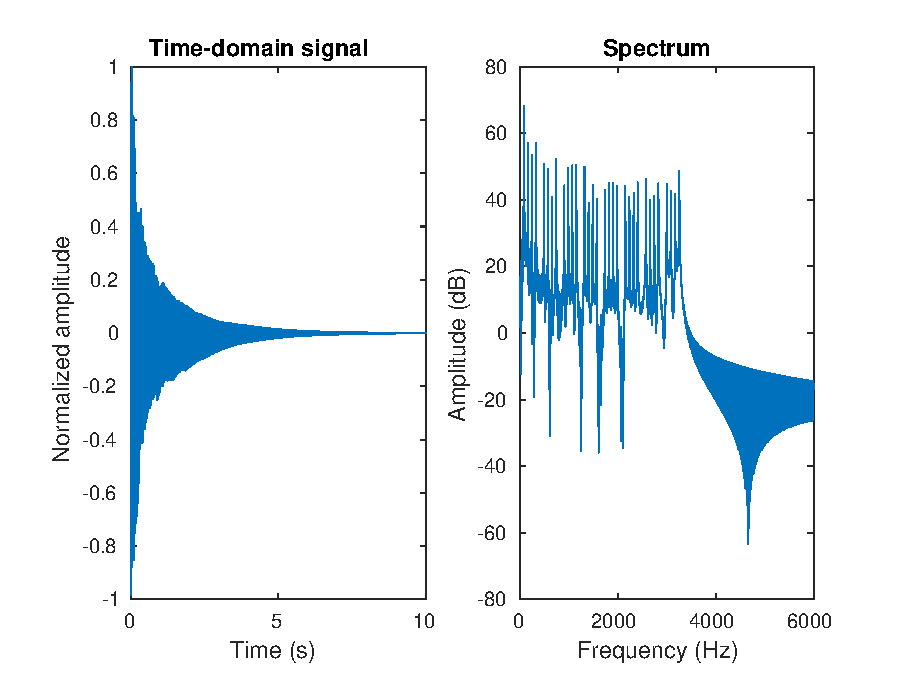
\includegraphics[scale=0.6]{figures/modal_synthesis-E2-40_string_modes-15_body_modes-finger_pluck.eps}
 \caption{Synthèse modale, \( E2 \), largeur de doigt, \( 40 \) modes de corps
 \label{fig:synth:modal_synth}}
\end{table}


\chapter*{Conclusion et discussion}


\printbibliography{}

\end{document}
